%\nonstopmode
\documentclass[12pt]{article}
%\documentclass{article}
\usepackage[utf8]{inputenc}
\usepackage{booktabs}% http://ctan.org/pkg/booktabs
\usepackage{multirow}
\usepackage{microtype}      % microtypography
\usepackage[a4paper, margin=0.78in]{geometry}
\newcommand{\argmax}{\operatornamewithlimits{\mathbb{argmax}}}
\usepackage{amssymb}
\usepackage{breqn}
\usepackage{bm}
\usepackage{wrapfig}
\usepackage{amsmath,eqnarray}
\usepackage[svgnames]{xcolor}
\definecolor{citecol}{RGB}{0,12,128}
\usepackage{bm}
\usepackage{graphicx}
\usepackage[subrefformat=parens,labelformat=parens]{subfig}
\usepackage{float}
\usepackage{mathptmx}
\usepackage[ruled,vlined,linesnumbered]{algorithm2e}
%\usepackage[backend=bibtex,style=alphabetic,citestyle=authoryear]{biblatex}
\usepackage[numbers]{natbib}
\bibliographystyle{abbrv}
% \usepackage{amsmath}
\usepackage{amsfonts}
% \usepackage{hyperref}
\usepackage{yhmath}
\usepackage{colortbl}
\newcommand{\tabitem}{~~\llap{\textbullet}~~}

\newcommand{\xhdr}[1]{{\noindent\bfseries #1}.}

\newcommand{\matr}[1]{\mathbf{#1}}
\newcommand{\vect}[1]{\mathbf{#1}}

\newcommand{\va}[0]{\vect{a}}
\newcommand{\vb}[0]{\vect{b}}
\newcommand{\vc}[0]{\vect{c}}
\newcommand{\vd}[0]{\vect{d}}
\newcommand{\ve}[0]{\vect{e}}
\newcommand{\vf}[0]{\vect{f}}
\newcommand{\vg}[0]{\vect{g}}
\newcommand{\vh}[0]{\vect{h}}
\newcommand{\vi}[0]{\vect{i}}
\newcommand{\vm}[0]{\vect{m}}
\newcommand{\vo}[0]{\vect{o}}
\newcommand{\vp}[0]{\vect{p}}
\newcommand{\vq}[0]{\vect{q}}
\newcommand{\vr}[0]{\vect{r}}
\newcommand{\vs}[0]{\vect{s}}
\newcommand{\vv}[0]{\vect{v}}
\newcommand{\vw}[0]{\vect{w}}
\newcommand{\vx}[0]{\vect{x}}
\newcommand{\vy}[0]{\vect{y}}
\newcommand{\vz}[0]{\vect{z}}


\newcommand{\mF}[0]{\matr{F}}
\newcommand{\mH}[0]{\matr{H}}
\newcommand{\mM}[0]{\matr{M}}
\newcommand{\mQ}[0]{\matr{Q}}
\newcommand{\mR}[0]{\matr{R}}
\newcommand{\mU}[0]{\matr{U}}
\newcommand{\mV}[0]{\matr{V}}
\newcommand{\mW}[0]{\matr{W}}

\def\Snospace~{\S{}} % If i don't add this overleaf complains
\renewcommand{\sectionautorefname}{\Snospace}
\renewcommand{\subsectionautorefname}{\Snospace}

%\hypersetup{colorlinks=true,citecolor=citecol}
%\DeclareMathOperator*{\argmax}{arg\,max}

%\addbibresource{syllabus.bib}

\title{Systematic language understanding: a study on the capabilities and limits of language understanding by modern neural networks}
\author{Koustuv Sinha \\ Ph.D. Proposal Document}
\date{September 2021}

\begin{document}

\maketitle

\section{Introduction}

Language allows us to express and comprehend a vast variety of novel thoughts and ideas. Through language, humans exhibit higher-order reasoning and comprehension. Thus, to develop models which mimic human-like reasoning, a principled focus in computer science research is to develop models which understand and reason on natural language. To foster research in developing such state-of-the-art natural language understanding (NLU) models, several datasets and tasks on reading comprehension have been proposed in recent literature. These include tasks such as question answering (QA), natural language inference (NLI), commonsense reasoning to name a few. Over the last decade, several advancements have been made to develop such models, the most successful ones till date involve deep neural models, especially Transformers \CITE, a class of multi-head self-attention models. Since its introduction in 2017, Transformer-based models have achieved impressive results on numerous benchmarks and datasets, with BERT \CITE being one of the most popular instantiation of the same. Using a technique known as ``pre-training'', Transformer-based models are first trained to replicate massive corpus of text. Through this kind of unsupervised training, the models learn and tune their millions and billions of parameters, and using which they solve NLU datasets with surprising, near-human efficiency \CITE.

While Transformer-based models excel in these datasets, it is less clear why do they work so well. Due to the sheer amount of overparameterization, direct inspection of the inner workings of these models are limited. Thus, various research have been conducted by using auxilliary tasks and probing functions to understand the reasoning processes employed by these models \cite{rogers2020}. It has been claimed in the literature that BERT embeddings contain syntactic information about a given sentence, to the extent that the model may internally perform several natural language processing pipeline steps, involving parts-of-speech tagging, entity recognition etc \CITE. BERT has also been credited to acquire some level of semantic understanding \CITE, and contains relevant information about relations and world knowledge \CITE. All of these results indicate to the fact that purely pre-training with massive overparameterized models and large corpora might just be the perfect roadmap to achieve ``human-like'' reasoning capabilities.

On the other hand, there have been growing concerns regarding the ability of these NLU models to understand language in a ``systematic'' and robust way. The phenomenon of \textit{systematicity}, widely studied in the cognitive sciences, refers to the fact that lexical units such as words make consistent contributions to the meaning of the sentences in which they appear \CITE[Fodor]. As an illustration, they provide an example that all English speakers who understand the sentence ``John loves the girl'' should also understand the phrase ``the girl loves John''. In case of NLU tasks, this accounts to model being consistent in understanding novel compositions of existing, learned words or phrases. However, there is growing evidence in literature which highlight the brittleness of NLU systems to such adversarial examples \CITE. More so, there is strong evidence that state-of-the-art NLU models tend to exploit statistical artifacts in datasets, rather than exhibiting true reasoning and generalization capabilities \CITE.

In view of the positive and negative evidences towards Transformers acquiring ``human-like'' natural language understanding capacity, it is very important that we take a step back and carefully examine the reasoning processes of the NLU models in the view of systematicity and robustness. Since these NLU models are now being deployed in production and decision making systems, it is even more prudent to test the models towards systematic understanding in order to avoid catastrophic scenarios. In this proposal, I thus discuss my work till now in my doctoral studies to understand the limits of systematic and robust natural language understanding of NLU models. Concretely, first I discuss our proposed systematicity tests on artificial and natural languages by using first-order logic (FOL), and what we learned from the model using such tests. This involves the following paper:

\begin{itemize}
  \item \textit{CLUTRR: A Diagnostic Benchmark for Inductive Reasoning from Text}, published at Empirical Methods of Natural Language Processing (EMNLP) 2019 (Oral presentation) \cite{sinha2019a}
\end{itemize}

This document does not discuss in detail about my other related works in this topic, such as in Natural Language Inference, \textit{Probing Linguistic Systematicity} \footnote{Work done as second author.}, published at Association for Computational Linguistics (ACL) 2020 \cite{goodwin2020}; or in proof generation, \textit{Measuring Systematic Generalization in Neural Proof Generation} \cite{gontier2020}, published at Neural Information Processing Systems (NeurIPS) 2020.

Secondly, I discuss our work on understanding the limits of systematicity of NLU models by subjecting these models to scrambled word order sentences, involving the following two papers:

\begin{itemize}
  \item \textit{UnNatural Language Inference}, published at Association for Computational Linguistics (ACL) 2021 (Oral presentation, Outstanding paper award) \cite{sinha2021}
  \item \textit{Masked Language Modeling and the Distributional Hypothesis: Order Word Matters Pre-training for Little}, published at Empirical Methods of Natural Language Processing (EMNLP) 2021 \cite{sinha2021a}
\end{itemize}

This document does not discuss concurrent works on analyzing faithfulness and robustness in translations \cite{parthasarathi2021a} (published at EMNLP 2021), proposed dataset on systematic reasoning on graph neural networks \cite{sinha2020c}, or an unreferenced automatic dialog evaluation framework \cite{sinha2020d} (published at ACL 2020) conducted during my doctoral studies.

% TODO mostly copy/rephrase stuff from my previous papers. Start with a general introduction

% TODO define systematicity

% TODO state why we need to investigate systematicity of NLU models - cite the problem papers

% Related work

% Connect systematicity to generalization

\section{Background}

% Language Models

\subsection{Language Models}

%Transformers
% LSTM-based LM

% The rise of pre-training

\subsection{The rise of pre-training}

\section{Contribution 1: Investigating systematicity of NLU models using first order logic}
\label{sec:cont1}

\subsection{Motivation}

An important challenge in NLU is to develop benchmarks which can precisely test a model's capability for robust and systematic generalization. Ideally, we want language understanding systems that can not only answer questions and draw inferences from text, but that can also do so in a systematic, logical and robust way. While such reasoning capabilities are certainly required for many existing NLU tasks, most datasets combine several challenges of language understanding into one, such as co-reference/entity resolution, incorporating world knowledge, and semantic parsing - making it difficult to isolate and diagnose a model's capabilities for systematic generalization and robustness.

\begin{wrapfigure}{r}{0.5\textwidth}
\begin{center}
  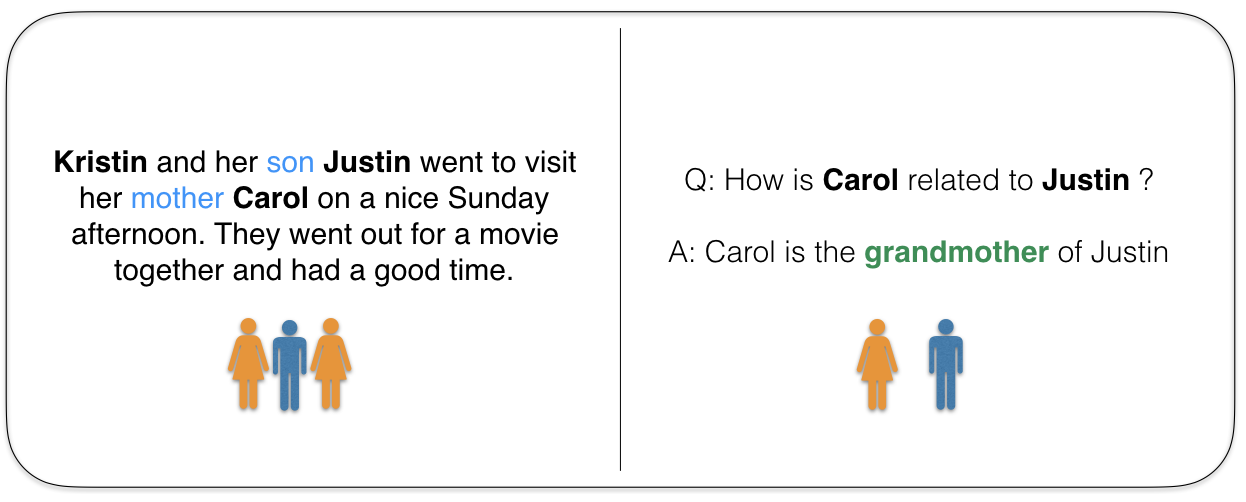
\includegraphics[width=0.48\textwidth]{images/clutrr_text.png}
\end{center}
\caption{CLUTRR inductive reasoning task}
\label{fig:clutrr_data}
\end{wrapfigure}



Thus, inspired by the classic AI challenge of inductive logic programming, we propose a semi-synthetic benchmark designed to explicitly test an NLU model's ability for systematic and robust logical generalization. Our benchmark suite - termed CLUTRR (Compositional Language Understanding with Text-based Relational Reasoning) - contains a large set of semi-synthetic stories involving hypothetical families. Given a story, the objective is to infer the relationship between two given characters in the story, whose relationship is not explicitly mentioned. To solve this task, a alearning agent must extract the relationships mentioned in the text, induce the logical rules governing the kinship relationships (e.g, the transitivity of the sibling relation), and use rules to infer the relationship between a given pair of entities.

\subsection{Dataset Design}

In order to design the CLUTRR benchmark, we build upon classic ILP task of inferring kinship relations. For example, given the facts that \textit{``Alice is Bob's mother''} and \textit{``Jim is Alice's father''}, one can infer with reasonable certainty that \textit{``Jim is Bob's grandfather''}. While this example may appear trivial, it is challenging task to design models that can learn from data to \textit{induce} the logical rules necessary to make such inferences, and it is even more challenging to design models that can systematically generalize by composing these induced rules. Thus, the core idea behind CLUTRR benchmark suite is the following: given a natural language story describing a set of kinship relations, the goal is to infer the relationship between two entities, whose relationship is \textit{not} explicitly stated in the story. To generate these stories, we first design a knowledge base (KB) with rules specifying how kinship relations resolve, and we use the following steps to create semi-synthetic stories based on this knowledge base:

\begin{itemize}
        \item \textbf{Step 1.} Generate a random kinship graph that satisfies the rules in our KB.
        \item \textbf{Step 2.} Sample a target fact (i.e relation) to predict from the kinship graph
        \item \textbf{Step 3.} Apply backward chaining to sample a set of $k$ facts that can prove the target relation (and optionally sample a set of ``distracting'' or ``irrelevant'' noise facts)
        \item \textbf{Step 4.} Convert the sampled facts into a natural language story through pre-specified text templates and crowd-sourced paraphrasing.
\end{itemize}

\begin{wrapfigure}{r}{0.5\textwidth}
\begin{center}
  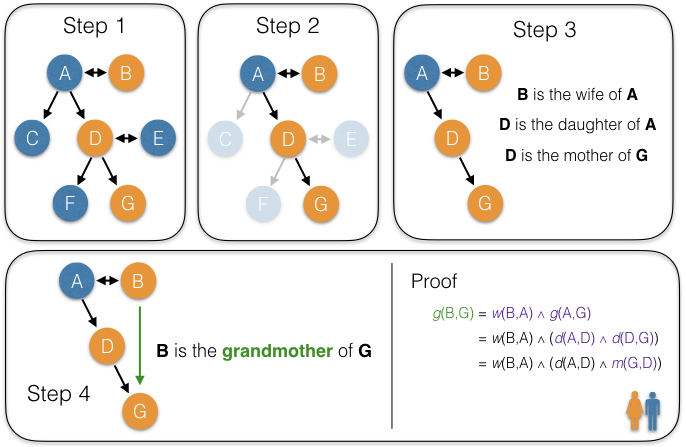
\includegraphics[width=0.48\textwidth]{images/clutrr_dataset_proof.png}
\end{center}
\caption{CLUTRR dataset design steps}
\label{fig:clutrr_data_design}
\end{wrapfigure}



Essentially, we use first order logic (FOL) to generate $k$ number of provable facts and then apply natural language layer on top of it to create a semi-synthetic benchmark. The number $k$ denotes the difficulty of the example. We use Amazon Mechanical Turk (AMT) crowd workers to annotate logical facts into narratives. Since workers are given a set of facts logical facts to work from, they are able to combine and split multiple facts across separate sentences and construct diverse narratives (Figure \ref{fig:clutrr_composition}).
One challenge for data collection via AMT is that the number of possible stories generated by CLUTRR grows combinatorially as the number of supporting facts increases. This makes it infeasible to obtain a large number of paraphrased examples. To circumvent this issue and increase the flexibility of our benchmark, we reuse and compose AMT paraphrases to generate longer stories.
In particular, we collected paraphrases for stories containing $k=1,2,3$ supporting facts and then replaced the entities from these collected stories with placeholders in order to re-use them to generate longer semi-synthetic stories.

\begin{wrapfigure}{r}{0.5\textwidth}
\begin{center}
  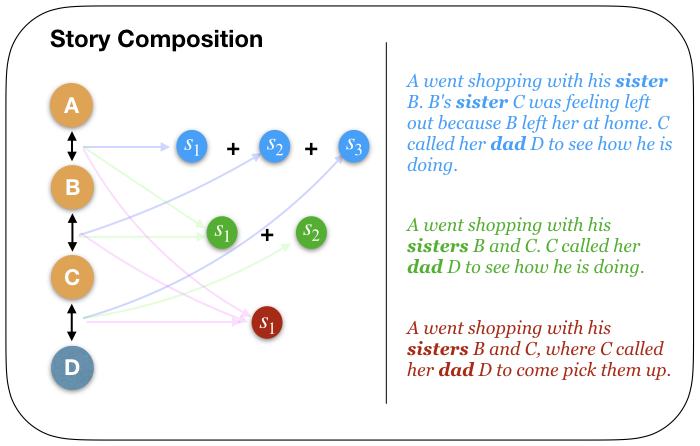
\includegraphics[width=0.48\textwidth]{images/clutrr_composition.png}
\end{center}
\caption{Generation of stories by composition in CLUTRR}
\label{fig:clutrr_composition}
\end{wrapfigure}



An example of a story generated by stitching together two shorter paraphrases is provided below:

\begin{quote}{\small
    [Frank] went to the park with his father, [Brett]. [Frank] called his brother [Boyd] on the phone. He wanted to go out for some beers.
    [Boyd] went to the baseball game with his son [Jim].\\
    Q: What is [Brett] and [Jim]'s relationship?}
\end{quote}

Thus, instead of simply collecting paraphrases for a fixed number of stories, we instead obtain a diverse collection of natural language templates that can be programmatically recombined to generate stories with various properties. Please refer to our paper \cite{sinha2019a} for more details about the data generation process.


\subsection{Experiments}

In this section, we use CLUTRR to construct specific instances of the dataset to test various aspects of systematicity in natural language understanding.
We report training and testing results on stories with different clause lengths $k$.
(For brevity, we use the phrase ``clause length'' throughout this section to refer to the number of steps of reasoning that are required to predict the target query.)
We also ensure the AMT templates are also split into train and test, to reduce the probability of overfitting to certain artifacts of the templates.

\xhdr{Human Performance} To get a sense of the data quality and difficulty involved in CLUTRR, we asked human annotators to solve the task for random examples of length $k=2,3,...,6$.
We found that time-constrained AMT annotators performed well (i.e., ${>70\%}$) accuracy for ${k\leq 3}$ but struggled with examples involving longer stories, achieving 40-50\% accuracy for ${k > 3}$. However, trained annotators with unlimited time were able to solve 100\% of the examples (Appendix 1.7), highlighting the fact that this task requires attention and involved reasoning, even for humans.

\xhdr{\textit{Are NLU models able to generalize systematically?}}

In this setup, we consider the setting where the models are trained on stories generated from clauses of length ${\leq k}$ and evaluated on stories generated from larger clauses of length ${>k}$. Thus, we explicitly test the ability for models to generalize on examples that require more steps of reasoning that any example they encountered during training.
In other words, during training, the model sees all logical rules but does not see all {\em combinations} of these logical rules.

\begin{wrapfigure}{l}{0.5\textwidth}
\begin{center}
  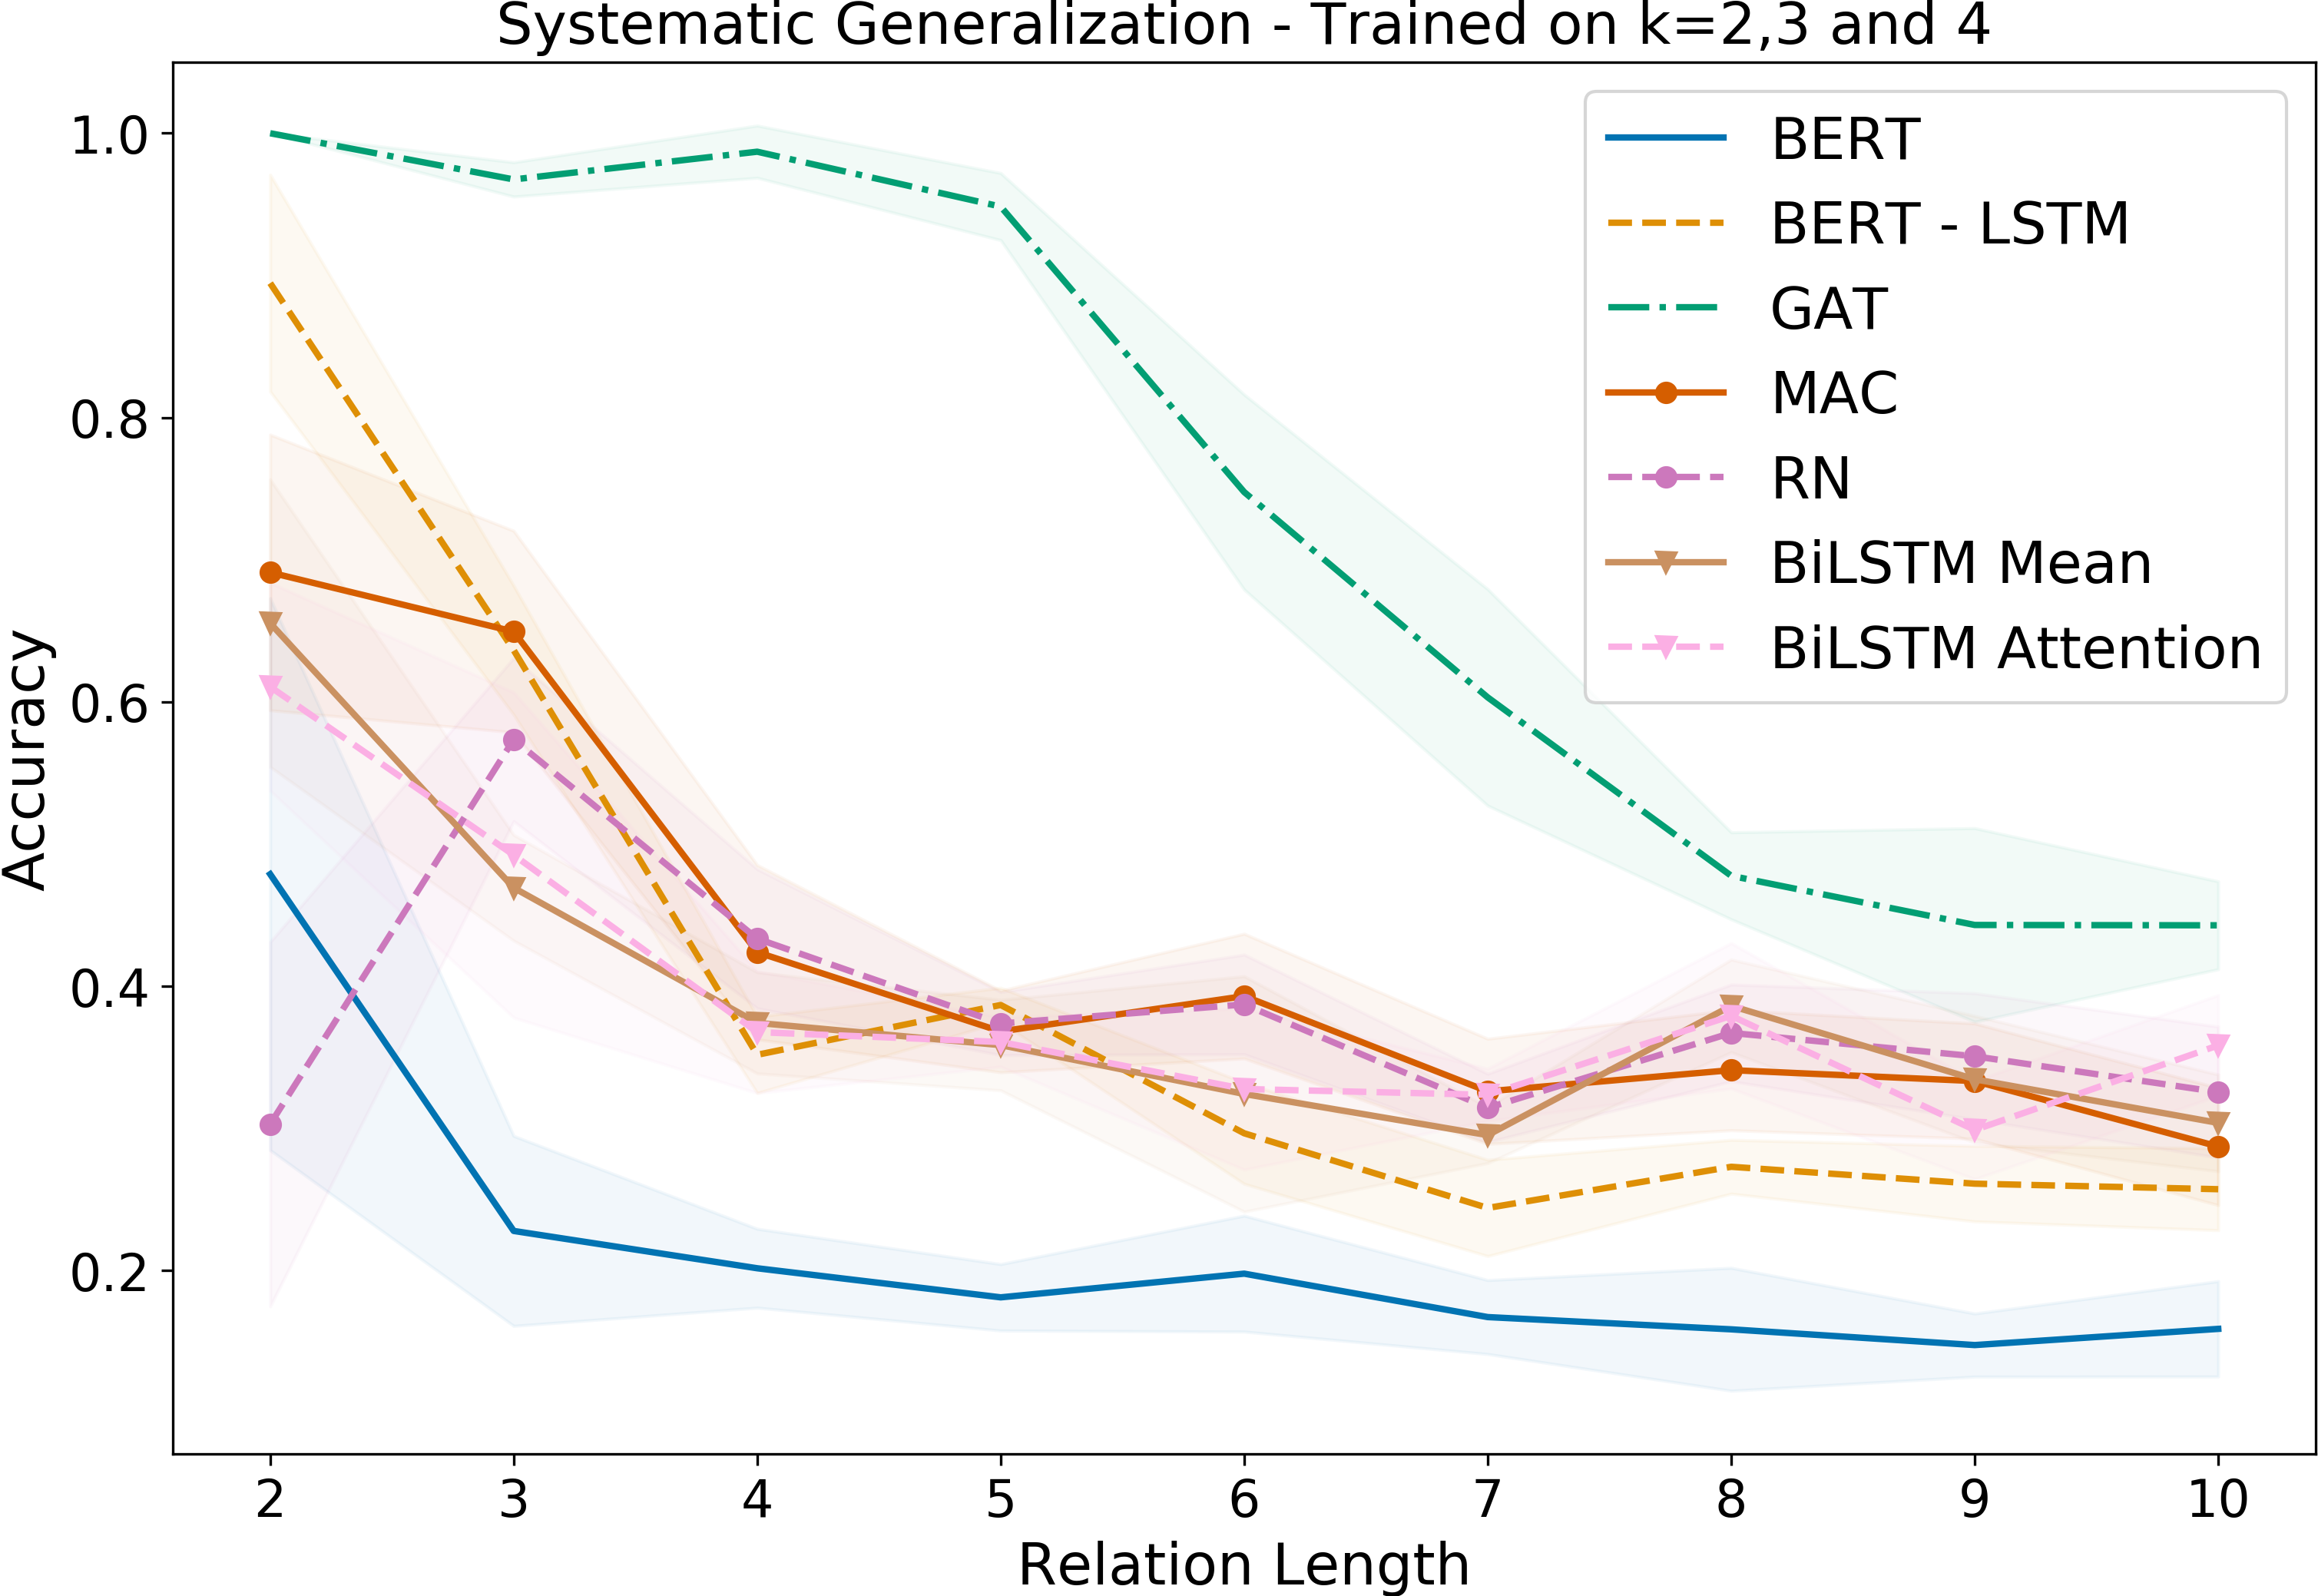
\includegraphics[width=0.48\textwidth]{images/clutrr_sys_gen_234.png}
\end{center}
\caption{Systematic generalization results on CLUTRR, when trained on stories of length $k=2,3,4$}
\label{fig:clutrr_sys_gen_234}
\end{wrapfigure}


Figure \ref{fig:clutrr_sys_gen_234} illustrates the performance of different NLU models on this generalization task. For NLU models, we consider bidirectional LSTMs \citep{hochreiter1997long, cho2014learning} (with and without attention), as well as recently proposed models that aim to incorporate inductive biases towards relational reasoning: Relation Networks (RN) \citep{santoro2017simple} and Compositional Memory Attention Network (MAC) \citep{hudson2018compositional}. We also use the large pretrained language model, BERT \cite{devlin2018bert}, as well as a modified version of BERT having a trainable LSTM encoder on top of the pretrained BERT embeddings. Since the underlying relations in the stories generated by CLUTRR inherently form a graph, we also experiment with a Graph Attention Network (GAT) \citep{Velickovic2017-mh}. Rather than taking the textual stories as input, the GAT baseline receives a structured graph representation of the facts that underlie the story.

We observe that the GAT model is able to perform near-perfectly on the held-out logical clauses of length $k=3$, with the BERT-LSTM being the top-performer among the text-based models but still significantly below the GAT.
Not surprisingly, the performance of all models degrades monotonically as we increase the length of the test clauses, which highlights the challenge of ``zero-shot'' systematic generalization \cite{lake2017generalization, 2018arXiv181107017S}.
GAT, having access to structured input, is able to generalize significantly better compared to NLU models.


% \xhdr{\textit{Is there any benefit to structured input for generalization?}}

% The empirical results on systematic generalization also provide insight into how the text-based NLU systems compare against the graph-based GAT model that has full access to the logical graph structure underlying the stories. Indeed, the relatively strong performance of the GAT model (Figure \ref{fig:gen_1}) suggests that the language-based models fail to learn a robust mapping from the natural language narratives to the underlying logical facts.

% To further confirm this trend, we ran experiments with modified train and test splits for the text-based models, where the same set of natural language paraphrases were used to construct the narratives in both the train and test splits (see our paper \cite{sinha2019a} for details). In this simplified setting, the text-based models must still learn to reason about held-out logical patterns, but the difficulty of parsing the natural language is essentially removed, as the same natural language paraphrases are used during testing and training. We found that the text-based models were competitive with the GAT model in this simplified setting, confirming that the poor performance of the text-based models on the main task is driven by the difficulty of parsing the unseen natural language narratives.


\xhdr{\textit{How does NLU systems cope with noise - how robustly do they reason?}}

Finally, we use CLUTRR to systematically evaluate how NLU models cope with noise.
Any set of supporting facts generated by CLUTRR can be interpreted as a path in the corresponding kinship graph $G$ (Figure \ref{fig:clutrr_data_noise}).

\begin{wrapfigure}{l}{0.5\textwidth}
\begin{center}
  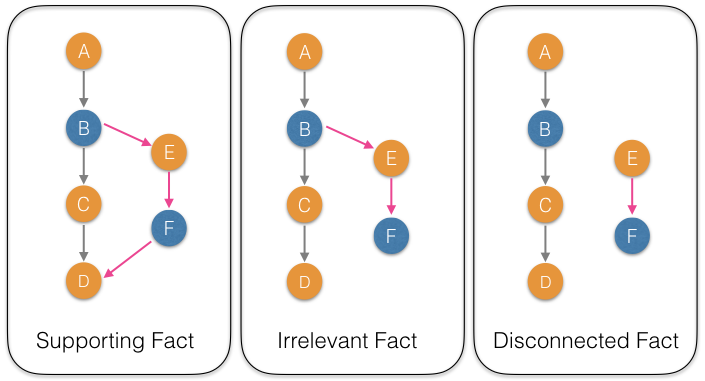
\includegraphics[width=0.48\textwidth]{images/clutrr_noise.png}
\end{center}
\caption{Noise generation methods in CLUTRR}
\label{fig:clutrr_data_noise}
\end{wrapfigure}

Based on this interpretation, we view adding noise facts to the \textit{clean path} from the perspective of sampling three different types of noise paths, from the kinship graph $G$:

\begin{itemize}
    \item \textit{Irrelevant facts}: We add a path, which has exactly one shared end-point with the clean path. In this way, this is a \textit{distractor} path,
    which contains facts that are connected to one of the entities in the target relation, but do not provide any information that could be used to help answer the query. %We name this task \texttt{CLUTRR-Irrelevant}
     \item \textit{Supporting facts}:
    We add a path whose two end-points are on the clean path.
    The facts on this path are noise because they are not needed to answer the query, but they are supporting facts because they can, in principle, be used to construct alternative (longer) reasoning paths that connect the two target entities.
    %We denote this setup as \texttt{CLUTRR-Supporting}
    \item \textit{Disconnected facts}: We add paths which neither originate nor end in any entity on the clean path. These disconnected facts involve entities and relations that are completely unrelated to the target query.
    %We call this variant \texttt{CLUTRR-Disconnected}.
\end{itemize}

\begin{table}[t!]
\caption{Testing the robustness of the various models when training and testing on stories containing various types of noise facts.}
\label{tab:robust}
\resizebox{\textwidth}{!}{
% Please add the following required packages to your document preamble:
% \usepackage{multirow}
\begin{tabular}{@{}cccccccc|c@{}}
\toprule
\multicolumn{1}{l}{} & \multicolumn{1}{l}{Models} & \multicolumn{6}{c}{Unstructured models (no graph)} & \multicolumn{1}{l}{Structured model (with graph)} \\ \midrule
\multicolumn{1}{l}{Training} & \multicolumn{1}{l|}{Testing} & BiLSTM - Attention & BiLSTM - Mean & RN & MAC & \multicolumn{1}{l}{BERT} & \multicolumn{1}{l|}{BERT-LSTM} & GAT \\ \midrule
Clean & \multicolumn{1}{c|}{Clean} & 0.58 \tiny $\pm 0.05$ & 0.53 \tiny $\pm 0.05$ & 0.49 \tiny $\pm 0.06$ & 0.63 \tiny $\pm 0.08$ & 0.37 \tiny $\pm 0.06$ & 0.67 \tiny $\pm 0.03$ & \textbf{1.0} \tiny $\pm 0.0$ \\
 & \multicolumn{1}{c|}{Supporting} & \textbf{0.76} \tiny $\pm 0.02$ & 0.64 \tiny $\pm 0.22$ & 0.58 \tiny $\pm 0.06$ & 0.71 \tiny $\pm 0.07$ & 0.28 \tiny $\pm 0.1$ & 0.66 \tiny $\pm 0.06$ & 0.24 \tiny $\pm 0.2$ \\
 & \multicolumn{1}{c|}{Irrelevant} & 0.7 \tiny $\pm 0.15$ & \textbf{0.76} \tiny $\pm 0.02$ & 0.59 \tiny $\pm 0.06$ & 0.69 \tiny $\pm 0.05$ & 0.24 \tiny $\pm 0.08$ & 0.55 \tiny $\pm 0.03$ & 0.51 \tiny $\pm 0.15$ \\
 & \multicolumn{1}{c|}{Disconnected} & 0.49 \tiny $\pm 0.05$ & 0.45 \tiny $\pm 0.05$ & 0.5 \tiny $\pm 0.06$ & 0.59 \tiny $\pm 0.05$ & 0.24 \tiny $\pm 0.08$ & 0.5 \tiny $\pm 0.06$ & \textbf{0.8} \tiny $\pm 0.17$ \\ \midrule
Supporting & \multicolumn{1}{c|}{Supporting} & 0.67 \tiny $\pm 0.06$ & 0.66 \tiny $\pm 0.07$ & 0.68 \tiny $\pm 0.05$ & 0.65 \tiny $\pm 0.04$ & 0.32 \tiny $\pm 0.09$ & 0.57 \tiny $\pm 0.04$ & \textbf{0.98} \tiny $\pm 0.01$ \\
\midrule
Irrelevant & \multicolumn{1}{c|}{Irrelevant} & 0.51 \tiny $\pm 0.06$ & 0.52 \tiny $\pm 0.06$ & 0.5 \tiny $\pm 0.04$ & 0.56 \tiny $\pm 0.04$ & 0.25 \tiny $\pm 0.06$ & 0.53 \tiny $\pm 0.06$ & \textbf{0.93} \tiny $\pm 0.01$ \\
\midrule
Disconnected & \multicolumn{1}{c|}{Disconnected} & 0.57 \tiny $\pm 0.07$ & 0.57 \tiny $\pm 0.06$ & 0.45 \tiny $\pm 0.11$ & 0.4 \tiny $\pm 0.1$ & 0.17 \tiny $\pm 0.05$ & 0.47 \tiny $\pm 0.06$ & \textbf{0.96} \tiny $\pm 0.01$ \\ \midrule
  \multicolumn{1}{l}{Average} & \multicolumn{1}{c|}{} & \textbf{0.61} \tiny $\pm 0.08$ & 0.59 \tiny $\pm 0.08$ & 0.54 \tiny $\pm 0.07$ & \textbf{0.61} \tiny $\pm 0.06$ & 0.30 \tiny $\pm 0.07$ & 0.56 \tiny $\pm 0.05$ & \textbf{0.77} \tiny $\pm 0.09$ \\ \bottomrule
\end{tabular}}
\end{table}


Overall, we find that the GAT baseline outperforms the unstructured text-based models across most testing scenarios (Table \ref{tab:robust}), which showcases the benefit of a structured feature space for robust reasoning.
When training on clean data and testing on noisy data, we observe two interesting trends that highlight the benefits and shortcomings of the various model classes:

\begin{enumerate}
    \item All the text-based models excluding BERT actually perform better when testing on examples that have {\em supporting} or {\em irrelevant} facts added. This suggests that these models actually benefit from having more content related to the entities in the story. Even though this content is not strictly useful or needed for the reasoning task, it may provide some linguistic cues (e.g., about entity genders) that the models exploit. In contrast, the BERT-based models do not benefit from the inclusion of this extra content, which is perhaps due to the fact that they are already built upon a strong language model (e.g., that already adequately captures entity genders.)
    \item  The GAT model performs poorly when {\em supporting} facts are added but has no performance drop when {\em disconnected} facts are added. This suggests that the GAT model is sensitive to changes that introduce cycles in the underlying graph structure but is robust to the addition of noise that is disconnected from the target entities.
\end{enumerate}
Moreover, when we trained on noisy examples, we found that only the GAT model was able to consistently improve its performance (Table \ref{tab:robust}).
Again, this highlights the performance gap between the unstructured text-based models and the GAT.

\subsection{Discussion}

In this paper we introduced the CLUTRR benchmark suite to test the systematic generalization and inductive reasoning capababilities of NLU systems.
We demonstrated the diagnostic capabilities of CLUTRR and found that existing NLU systems exhibit relatively poor robustness and systematic generalization capabilities---especially when compared to a graph neural network that works directly with symbolic input.
These results highlight the gap that remains between machine reasoning models that work with unstructured text and models that are given access to more structured input.
We hope that by using this benchmark suite, progress can be made in building more compositional, modular, and robust NLU systems.

\subsection{Related Works}

We also conduct a couple of related studies in testing systematicity of Natural Language Understanding (NLU) and Natural Language Generation (NLG) models following the intuition gained from CLUTRR.

\xhdr{\textit{Probing Linguistic Systematicity}} \cite{goodwin2020} In this work, we introduce several novel probes for testing systematic generalization in Natural Language Inference (NLI). Systematicity is the property whereby words have consistent contributions to composed meaning of the sentences. In this work, we employed an artificial, controlled language where we use \textit{Jabberwocky}-type \footnote{Jabberwocky is the term coined by Lewis Caroll in his poem, which combibes nonsense words with familiar words in a way that allows speakers to recognize the expression as well formed.} sentences to inspect the generalizability of word representations learned by neural networks. We gradually and systematically expose the NLU model to new, \textit{open-class} words in context of NLI tasks, and test whether this exposure alters the systematic understanding of existing, known \textit{closed-class} words. For example, we might train an NLI models with the premise-hypothesis contradiction pair \textit{All pigs sleep; some pigs don't sleep}, and test whether the network can identify the contradiction pair \textit{All Jabberwocks flug; some Jabberwocks don't flug}. A systematic learner would reliably identify the contradiction, whereas a non-systematic learner may allow the closed-class words (\textit{all, some, don't}) to take contextually conditioned meanings that depend on novel context words.

\begin{table*}[h]
  \centering
  \resizebox{\textwidth}{!}{
    \begin{tabular}{|l||llllll|}
      \hline
        \textbf{Position} & 1 & 2 & 3 &  4 & 5 & 6 \\ \hline
  \rowcolor{gray!6} \textbf{Category} & \texttt{quantifier} & \texttt{nominal premodifier} & \texttt{noun} &  \texttt{nominal postmodifier} & \texttt{negation} & \texttt{verb}  \\
  \textbf{Status} & Obligatory & Optional & Obligatory &  Optional & Optional & Obligatory\\
  \rowcolor{gray!6} \textbf{Class} & Closed & Closed & Open & Closed & Closed & Open \\
  \textbf{Example} & {\Large \exam{All}} &  {\Large \exam{brown}} &  {\Large  \exam{dogs}} &  {\Large  \exam{that bark}} &  {\Large \exam{don't}} &  {\Large \exam{run}} \\
  \hline
\end{tabular}
}
\caption{A template for sentences in the artificial language. Each sentence fills the obligatory positions 1, 3, and 6 with a word: a quantifier, noun, and verb. Optional positions (2, 4 and 5) are filled by either a word (adjective, postmodifier or negation) or by the empty string. Closed-class categories (Quantifiers, adjectives, post modifiers and negation) do not include novel words, while  open-class categories (nouns and verbs) includes novel words that are only exposed in the test set.
} \label{tbl:artlang}
\end{table*}


Concretely, we construct an artificial language with six-position template which includes a quantifier (position 1), noun (position 3), and a verb (position 6) with options pre- and post-modifiers (position 2 and 4) and optional negation (position 5). To mimic real world topicality, we contruct \textit{block} structures consisting of nouns and verbs having taxonomic relationships (such as \textit{lizards/animals. run/move}). Nouns and verbs from different blocks have no relationships (such as \textit{lizards} and \textit{screwdrivers} or \textit{run} and \textit{read}). The same set of closed-class words appear in all blocks with consistent meanings. We analyze several state-of-the-art NLI models such as Bidirectional LSTM, InferSent, self-attentive sentence encoder (SATT) and Hierarchical Convolutional Networks (CONV) \footnote{Since the first version of the paper was done prior to the popularity of BERT, we were unable to test the systematicty of BERT-based models in this work. However, our database and code are online, and it would be trivial to use pre-trained BERT models to run the same experiments.}.

We observed all models to perform substantially worse on probing tasks, with standard deviation being significantly high among various blocks - indicating unsystematic behavior. Closed-class words do not maintain a consistent intepretation when paired with different open-class words. Variance across blocks shows that under all models the behaviour of closed-class words is highly sensitive to the novel words they appear with. Thus, our experiments highlight that fact their despite high overall performance, state-of-the-art NLU models generalize in ways that allow the meanings of individual words to vary in different contexts, even in an artificial language where a totally systematic solution is available.

\xhdr{\textit{Measuring Systematic Generalization in Neural Proof Generation with Transformers}} \cite{gontier2020} In this work, we extend our systematicity analysis to language generation using Transformer Language Models (TLMs). To analyze systematicity, we re-use our CLUTRR benchmark to conduct proof generation using forward and backward chaining concepts in first-order logic (FOL). For example, a set of facts in CLUTRR could be of the form: \textit{``Nat is the granddaughter of Betty'', ``Greg is the brother of Nat'', ``Flo is the sister of Greg''}, where the relationship among \textit{Flo} and \textit{Betty} can be inferred using logical deduction (\textit{``Flo is the granddaughter of Betty''}). In this example, we further task the TLM to generate a plausible proof along with the answer : \textit{``Since Flo is the sister of Greg, and Nat is the granddaughter of Betty, and Greg is the brother of Nat, then Flo is the granddaugher to Betty''}.

In our work, we evaluate two popular proof resolution strategies used in Inductive Logic Programming \CITE[Evans], \textit{forward} and \textit{backward} chaining resolution paths, expressed in natural language. We evaluate the validity of the proof and the answer accuracy on various settings: whether the TLM is tasked to generated forward or backward proofs, whether the TLM is provided with a gold proof, or when the TLM is neither provided nor tasked to generate a proof. We train a Transformer \CITE[Vaswani] model on scratch on the training set, and we observe that TLMs are only able to generalize to unseen proof steps in case of \textit{interpolation}, that is when stories of lesser difficulties than training are provided during inference. In case of \textit{extrapolation}, we observe similar generalization issues as in CLUTRR, where models fail to generalize beyond the difficulty trained. In terms of proof understanding, we observed backward chaining proofs are better understood by the model than forward chaining for the TLMs, mostly due to the fact that backward chaining proofs always begings with the target answer first, allowing the model to exploit the positional cues. Surprisingly, we found the no proof situation to have better answer accuracy than in the case of proof generation - alluding to the fact that proof generation might be actually deterioriating the model performance as it requires more involved reasoning.

\begin{wrapfigure}{l}{0.5\textwidth}
\begin{center}
  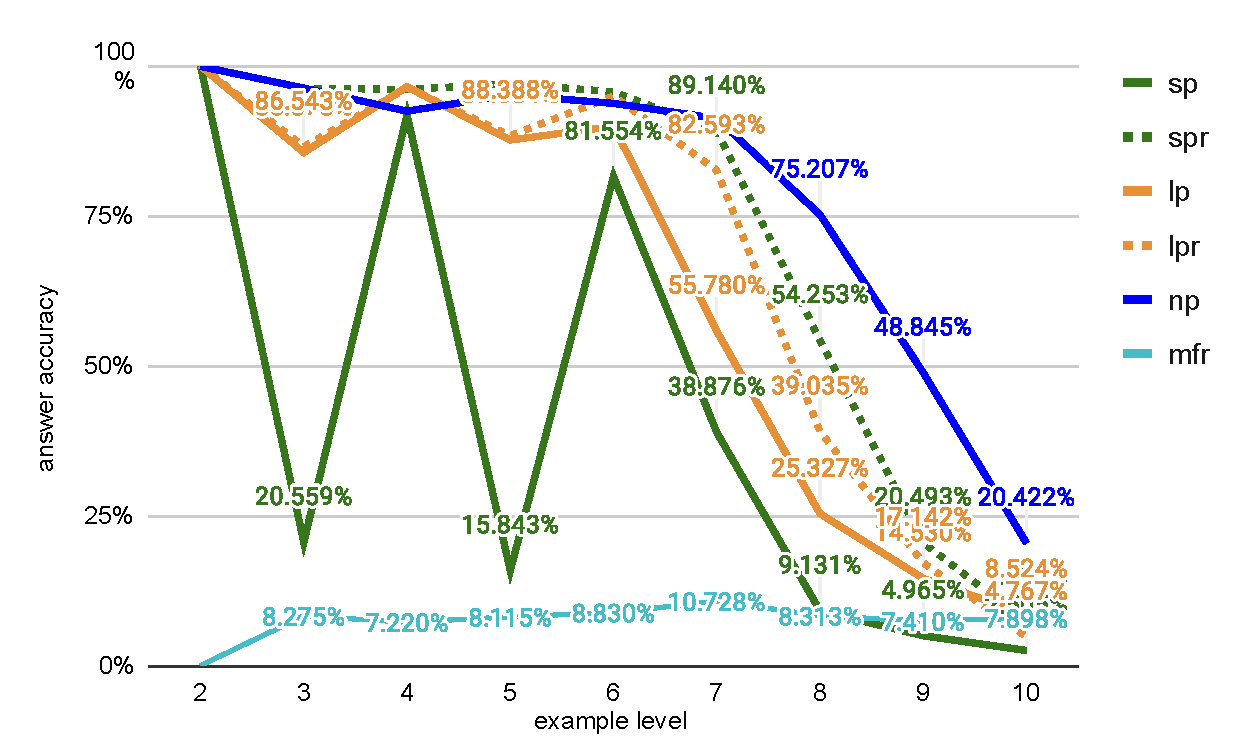
\includegraphics[width=0.48\textwidth]{images/proof_sys_gen.pdf}
\end{center}
\caption{Systematic generalization issues in proof generation}
\label{fig:proof_sys_gen}
\end{wrapfigure}


Finally, in proof generation, we found forward-chaining generation is easier for TLM than backward chaining generation. This is contrary to our previous observation, and we believe this is due to the fact that the model has a higher chance of generating the first proof step correctly than the final proof step. Overall, TLMs are unable to generate valid proofs of unseen lengths, both in \textit{interpolation} and \textit{extrapolation} setting. However, when provided with the correct proof, TLMs are better able to exploit the information in it to be better at systematic generalization. Our results highlight multiple insights - first, TLMs suffer length generalization issues in proof generation, and TLMs get better at reasoning when provided with correct proofs. Our framework can thus be used to easily analyze systematicity issues in generation as it is grounded with first-order logic.

\section{Contribution 2: Probing systematicity of pre-trained models using word order}
\label{sec:cont2}

% UNLI
% Unnatural Pre-training

Here, we talk about two related contributions, UnNatural Language Inference \cite{sinha2021} and pretraining with unnatural languages \cite{sinha2021a}.

\subsection{UnNatural Language Inference}

\subsection{Pre-training with Unnatural Languages}

\section{Future Work \& Timeline}

Until now, most of the work in my doctoral studies have been focused on developing methods to detect the issue of systematicity plaguing neural NLU models. To complete my thesis, I thereby plan to work towards a couple of methods to improve robustness and systematicity of NLU models.

\subsection{Unsupervised syntax learning by mutually exclusive training using word order}

In our prior work on word order (Section \ref{sec:cont2}), we observed that NLU models are largely distributional - they understand the collection of words in a sentence but have limited understanding on the order of words. This poses a problem - representations of random permutations of the sentence having no grounded meaning will still be identified by the NLU models to contain syntactic and semantic information. Due to this distributional effect, we posit that syntax understanding of NLU models are still primitive, mostly restricted to higher order information. Thus, it is imperative to develop mechanisms to imbibe the required syntactical information within the sentence representation, such that it is systematic. One can use syntactic features such as dependency parses to imbibe information about syntax in the sentence representation using auxilliary supervison loss. In literature, such syntactical information has shown to be effective in downstream tasks, such as Relation Extraction (RE) \cite{fundel2007relex}, named entity recognition (NER) \cite{jie2019dependency} and semantic role labeling (SRL) \cite{strubell2018}. More recently, syntax trees are used during pre-training of Transformer based models to imbibe better syntactical information by early and late fusion \cite{sachan2021}. However, such direct supervision models to imbibe syntactical information is difficult as it requires access to preferably human-annotated syntax parses of sentences, which raises questions on the viability of such approaches for real world applications. Even so, limited studies have been performed to investigate systematicity issues of those models trained with supplementary syntactical signal.

Therefore, we propose an alternate, unsupervised mechanism to imbibe syntax information within the sentence representations by leveraging word order. Concretely, we use an auxilliary objective to the model to recognize correct and incorrect permutations of a given sentence alongside the task objective. Now, in the strictest sense there is only one correct ordering of a sentence which conveys the intended meaning. However, natural language (English) allows for a degree of flexibility in word order. Thus, we plan to leverage the idea of \textit{separable permutations} \cite{stanojevic2021}, where a subset of permutations can be treated as positive signal which can be reconstructed from the CCG parse of the given sentence. This auxilliary training loss could potentially inform the model to be systematic in understanding syntax, and thereby reduce the distributional, bag-of-words behavior of the encoder representations.

% Note: potential question from comittee: While this approach still requires a CCG parser, due to the nature of separable permutations this parser need not be perfect.

\subsection{Nonsensical data augmentation for better systematic generalization}

Systematic generalization is an issue which plagues many NLU tasks, in particular Natural Language Inference (NLI). Generalization to out-of-domain examples is poor \cite{nie2020}, and it has been shown that these models leverage the statistical artifacts in NLI datasets, such as SNLI and MNLI \cite{gururangan2018a}. One reason why models tend to overfit on the training data is the exposure bias to specific nouns/verbs/entities during training. When subjected to systematic stress test, the NLU models tend to be brittle as they fail to learn syntax of the training signal by fixating on the rare words and artifacts. Thus, we propose a dynamic data augmentation training scheme for NLU models where we repeat the training examples with word replacements from the same syntactic family. Overall, a sentence might lose its intended meaning (hence, ``nonsensical'') - however if the same operation is conducted on the premise, the entailment logic remains unchanged. Concretely, given a lexical item in a sentence, we randomly replace that item with another belonging to the same syntactic family, equally in both premise and hypothesis sentences. For empirical reasons we will restrict this replacement to specific family of lexicons (proper nouns, verbs) which typically form as rare elements in the dataset. We also plan to include a probabilistic model for this replacement which replaces lexicons based on their corpus probability to ensure uniformity in training. By systematically replacing the lexicons in a different context one can potentially increase the training data to reduce exposure bias problem. Similar methods have been devised for mitigating gender bias previously in the literature with varying success \cite{maudslay2020b}.

\subsection{Timeline}

\noindent \textbf{Unsupervised syntax learning by mutually exclusive training using word order} (1) Investigate CCG parsing to generate separable permutations on the fly, (2) Representational analysis on separable and non separable permutations, (3) Train auxillary loss with either direct supervision or partial gradient based methods such as Meta Learning, (4) Write paper for ACL 2022 or TACL 2022

\halfblankline

\noindent \textbf{Nonsensical data augmentation for better systematic generalization} (1) Investigate lexicon replacements by using syntactic parsers in a given dataset, (2) Analyze how the distribution of rare elements change in the training corpus by using this kind of replacement, (3) Test on out-of-domain data and NLI stress test sets, such as HANS \cite{mccoy2019}, (4) Write paper for EMNLP 2022.

\halfblankline

\noindent \textbf{Thesis preparation and submission} Expected defense date: Fall 2022

% Table if needed
% \begin{table}
% \centering
% \begin{tabular}{p{5cm}p{7cm}p{3cm}}
% Project & Task & Timeline\\
% \toprule
% Unsupervised syntax learning by mutually exclusive training using word order & \tabitem Investigate CCG parsing to generate separable permutations on the fly & \\
%  & \tabitem Representational analysis on separable and non separable permutations & \\
%  & \tabitem Train auxillary loss with either direct supervision or partial gradient based methods such as Meta Learning & \\
%  & \tabitem Write paper for ACL 2022 or TACL 2022 & \\
% Nonsensical data augmentation for better systematic generalization & \tabitem Investigate lexicon replacements by using syntactic parsers in a given dataset & \\
%  & \tabitem Analyze how the distribution of rare elements change in the training corpus by using this kind of replacement & \\
%  & \tabitem Test on out-of-domain data and NLI stress tests, such as HANS & \\
%  & \tabitem Write paper for EMNLP 2022 & \\
% \end{tabular}
% \end{table}


\bibliography{main}

\end{document}
